\section{Theorie}
\label{sec:Theorie}
\subsection{Gedämpfte Schwingung}
Ein ungedämpfter Schwingkreis besteht aus zwei Energiespeichern: eine Kapazität C
in Form eines Kondensators und eine Induktivität L in Form einer Spule. Befindet
sich Energie in dem System, so fliesst der Strom periodisch wechselnd von der
Kapazität zur Induktivität und umgekehrt. In einem idealen System bleibt die Energie
dabei erhalten.
Fügt man diesem Schwingkreis einen ohmschen Widerstand R hinzu, so erhält man eine
gedämpfte Schwingung, da an dem Widerstand kontinuierlich Energie als Joulsche Wärme
abfällt. Infolgedessen nehmen die Amplitude des Stroms und die Spannung am
Kondensator mit der Zeit ab. Ein solcher gedämpfter Schwingkreis ist in Abbildung
\ref{fig:gedaempfter_schwingkreis} zu sehen.
\begin{figure}
  \centering
  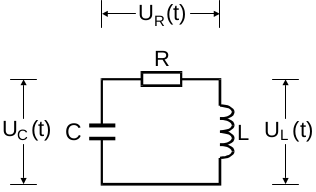
\includegraphics[width=0.6\textwidth]{gedaempfter_schwingkreis.png}
  \caption{Gedämpfter Schwingkreis mit einer Kapazität C, einem ohmschen Widerstand R
  und einer Induktivität L in einer Reihenschaltung \cite{sample}}
  \label{fig:gedaempfter_schwingkreis}
\end{figure}
Aus der Maschenregel der Kirchhoffschen Gesetze folgt, dass sich die drei Spannungen
$U_\symup{R} = R I$, $U_\symup{C} = \frac{Q}{C}$ und $U_\symup{L} = L \dot{I}$
sich zu Null addieren. Da $I=\dot{Q}$ gilt, ergibt sich die Differentialgleichung
einer gedämpften Schwingung zu
\begin{equation}
  \ddot{I} + \frac{R}{L}\dot{I} + \frac{1}{L C} I = 0.
  \label{eqn:dgl1}
\end{equation}
Dies ist eine homogene, lineare Differentialgleichung 2. Ordnung, die sich durch
den Ansatz
\begin{equation}
  I(t) = A e^{i \omega t}
  \label{eqn:ansatz}
\end{equation}
lösen lässt. Für $\omega$ ergibt sich
\begin{equation}
  \omega_{1,2} = i \frac{R}{2L}\pm \sqrt{\frac{1}{L C} - \frac{R^2}{4L^2}}.
  \label{eqn:omega12}
\end{equation}
Führt man die Abkürzungen
\begin{align*}
  \mu &= \frac{R}{4 \pi L} \text{ und }
  \nu &= \frac{1}{2\pi} \sqrt{\frac{1}{L C} - \frac{R^2}{4 L^2}}
\end{align*}
ein, erhält man alle Lösungen mit dem Superpositionsprinzip als
\begin{equation}
  I(t) = e^{-2 \pi \mu t} (u_1 e^{i 2 \pi \nu t} + u_2 e^{-i 2 \pi \nu t}).
  \label{eqn:loesung}
\end{equation}
Abhängig davon, ob $\frac{1}{L C}$ größer oder kleiner als $\frac{R^2}{4L^2}$ ist,
treten zwei Fälle auf: \newline
Fall 1: $\frac{1}{L C} > \frac{R^2}{4L^2}$, $\nu$ wird also reell. Dann müssen
die Konstanten $u_1$ und $u_2$ zueinander komplex konjungiert sein und mit der
Eulerschen Formel
\begin{equation}
  e^{i\phi} = \cos{\pi} + i \sin{\pi}
  \label{eqn:euler}
\end{equation}
folgt aus Gleichung \eqref{eqn:loesung}
\begin{equation}
  I(t) = A_0 e^{-2\pi\mu t}\cos{(2\pi\nu t + \eta)}.
  \label{eqn:gedaempfte_schwingung}
\end{equation}
Für diese Bedingung erhält man also eine gedämpfte, harmonische Schwingung mit der
Frequenz $\nu$.
\begin{figure}
  \centering
  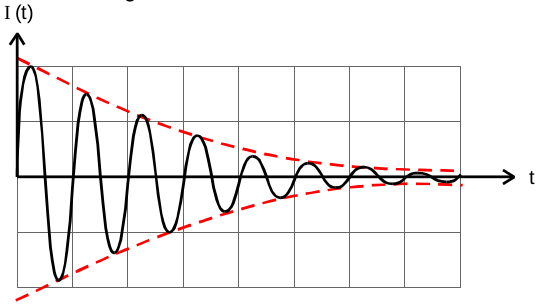
\includegraphics[width=0.6\textwidth]{gedaempfte_schwingung.png}
  \caption{Darstellung einer gedämpften Schwingung (rote Kurve), deren Einhüllenden
  (gestrichelte Kurven) durch die Funktionen $f(t)=\pm e^{-2\pi\mu t}$ gegeben
  sind \cite{sample}.}
  \label{fig:gedaempfte_schwingung}
\end{figure}
Die Amplitude der Schwinung geht wegen des Dämpfungsterms
$e^{-2\pi\mu t}$ für größer werdendes $t$ gegen Null. Die Periode der Schwinung
beträgt
\begin{equation}
  T = \frac{2\pi}{\sqrt{\frac{1}{L C}-\frac{R^2}{4 L^2}}}
  \label{eqn:periode}
\end{equation}
und die Abklingdauer $T_\symup{ex}$, also die Zeit, nach der die Amplitude auf den
e-ten Teil des Startwertes abgefallen ist, ist durch
\begin{equation}
  T_\symup{ex} = \frac{1}{2\pi\nu} = \frac{2L}{R}
  \label{eqn:abklingzeit}
\end{equation}
gegeben. In Grafik \ref{fig:gedaempfte_schwingung} ist ein solcher Schwingfall,
also eine gedämpfte Schwinung mit den einhüllenden Funktionen $f(t)=\pm e^{-2\pi\mu t}$,
die den exponentiellen Abfall vorgeben, zu sehen.


Fall 2: $\frac{1}{L C} < \frac{R^2}{4L^2}$, $\nu$ wird also imaginär. Dadurch heben
sich die imaginären Anteile der Schwingungsgleichung \eqref{eqn:loesung} gegenseitig
auf, so dass nur noch reele Exponentialfunktionen vorkommen und keine Schwingung
mehr auftritt. Dies entspricht einer aperiodischen Dämpfung, wie sie in Graifk
\ref{fig:ap_grenzfall} zu sehen ist. Je nach Wahl der Parameter kann erst ein Maximum
erreicht werden, bevor die Funktion exponentiell gegen Null abfällt. Diese Fälle
sind in der Grafik \ref{fig:ap_grenzfall} mit der roten und der blauen Kurve
dargestellt. Es kann auch ein Überschwingen, wie es in Grafik \ref{fig:ap_grenzfall}
mit der grünen Kurve zu sehen ist, auftreten.
Aus der Anfangsbedingung $\nu=0$ resultiert der sogenannte aperiodische Grenzfall,
bei dem gilt:
\begin{equation}
  \frac{1}{L C} = \frac{R_{\text{ap}}^2}{4 L^2} \iff I(t) = A e^{-\frac{1}{\sqrt{L C}}}.
  \label{eqn:bedingung-ap-grenzfall}
\end{equation}
Der aperiodische Grenzfall ist in Grafik \ref{fig:ap_grenzfall} mit der gestrichelten
Kurve dargestellt. Er beschreibt den Fall, bei dem $I(t)$ am schnellsten gegen Null
geht, jedoch ohne ins Negative überzuschwingen.
\begin{figure}
  \centering
  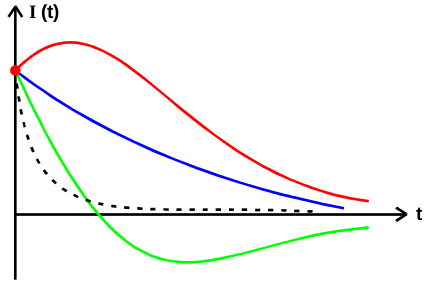
\includegraphics[width=0.6\textwidth]{ap_grenzfall.png}
  \caption{Dargestellt sind verschiedene Möglichkeiten des zeitlichen Verlaufs des
  Stromes bei aperiodischer Dämpfung, die gestrichelte Kurve beschreibt dabei den
  aperiodischen Grenzfall \cite{sample}.}
  \label{fig:ap_grenzfall}
\end{figure}

\subsection{Erzwungene Schwinung}
Wird an den Schwingkreis eine äußere periodische Spannung angelegt, führt dies zu
einer erzwungenen Schwinung. Eine schematische Darstellung einer erzwungenen
Schwingung ist in Abbildung \ref{fig:erz_schwingung} zu sehen.
\begin{figure}
  \centering
  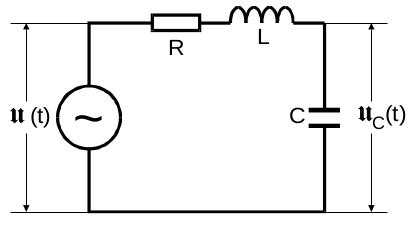
\includegraphics[width=0.6\textwidth]{erzwungene_schwingung.png}
  \caption{Eine Spannungsquelle führt dem gedämpften Schwingkreis eine sinusförmige
  Wechselspannung zu, sodass eine erzwungene Schwingung entsteht \cite{sample}.}
  \label{fig:erz_schwingung}
\end{figure}
Die von außen angelegte Spannung führt zu einer Inhomogenität in der Differentialgleichung
\eqref{eqn:dgl1}, welche nun
\begin{equation}
  L C \ddot{U_\symup{C}} + R C \dot{U_\symup{C}} + U_\symup{C} = U_0 e^{i\omega t}
  \label{eqn:dgl2}
\end{equation}
lautet. Als Lösung für die Spannung am Kondensator in Abhängigkeit von der Zeit
erhält man
\begin{equation}
  U(t) = \frac{U_0 (1 - L C \omega^2 - i \omega R C)}{(1 - L C \omega^2)^2 +
  \omega^2 R^2 C^2}.
  \label{eqn:loesung2}
\end{equation}
Die Phasenverschiebung zwischen Kondensatorspannung und Erregerspannung berechnet
sich durch
\begin{equation}
  \phi(\omega)=\arctan{\frac{Im(U)}{Re(U)}}
  = \arctan{\frac{-\omega R C}{1-L C \omega^2}}.
  \label{eqn:phasenverschiebung}
\end{equation}
Dieser Gleichung \eqref{eqn:phasenverschiebung} kann man entnehmen, dass die
Spannungen für kleine Frequenzen $\omega$ in Phase sind und für große Frequenzen
eine Phasenverschiebung von $\pi$ haben. Bei $\omega_0=\sqrt{\frac{1}{L C}}$ gilt
$\phi = -\frac{\pi}{2}$.\newline
Die Kondensatorspannung in Abhänigkeit der Erregerfrequenz $\omega$,
Resonanzkurve genannt, wird durch
\begin{equation}
  U_\symup{C}(\omega) = \frac{U_0}{\sqrt{(1-L C \omega^2)^2 + \omega^2 R^2 C^2}}.
  \label{eqn:resonanzkurve}
\end{equation}
berechnet. Betrachtet man das Verhalten von $U_\symup{C}(\omega)$ für bestimmte
$\omega$, so stellt man fest, dass $U_\symup{C}$ für $\omega \to \infty$ gegen
Null geht und für $\omega \to 0$ gegen $U_0$. Bei der Resonanzfrequenz
\begin{equation}
  \omega_\symup{res} = \sqrt{\frac{1}{L C}-\frac{R^2}{2L^2}}
  \label{eqn:resonanzfrequenz}
\end{equation}
erreicht $U_\symup{C}$ ein Maximum, welches größer als $U_0$ sein kann.
Es muss nun wieder zwischen zwei Fällen unterschieden werden:\newline
Wenn $\frac{1}{L C} \gg \frac{R^2}{2 L^2}$ ist, handelt es sich um schwache Dämpfung.
In diesem Fall nähert sich $\omega_\symup{res}$ $\omega_0$ an. Im Maximum nimmt
$U_C$ dann den Wert
\begin{equation}
  U_\symup{C,max} = \frac{1}{\omega_0 R C} U_0
  \label{eqn:Ucmax}
\end{equation}
an. Der Faktor $\frac{1}{\omega_0 R C}$ ist dabei die Resonanzüberhöhung oder
Güte $q$ des Schwingkreises. Geht $R$ jetzt gegen 0, so steigt $U_\symup{C,max}$
ins Undendliche, was dem Fall einer Resonanzkatastrophe entspricht.
Die Breite der Resonanzkurve bestimmt dabei die Schärfe der Resonanz. Man berechnet
für die Güte die Frequenzen $\omega_+$ und $\omega_-$, bei denen $U_\symup{C}$ auf
\begin{equation}
  \frac{1}{\sqrt{2}}U_\symup{C,max}
  \label{eqn:U0durchwurzel2}
\end{equation}
abgefallen ist.
Da $\frac{R^2}{L^2} \ll \omega_0^2$ gilt, folgt für die Breite der Resonanzkurve
mit Gleichung \eqref{eqn:U0durchwurzel2}
\begin{equation}
  \omega_+ - \omega_- \approx \frac{R}{L}.
  \label{eqn:breite_resonanzkurve}
\end{equation}
Für die Güte erhält man dann
\begin{equation}
  q = \frac{\omega_0}{\omega_+ + \omega_-}.
  \label{eqn:guete}
\end{equation}
Für den Fall der starken Dämpfung, also $\frac{1}{L C} \ll \frac{R^2}{2 L^2}$, tritt
keine Resonanzüberhöhung mehr ein. $U_\symup{C}$ geht von $U_0$ monoton fallend
gegen Null. Dieser Fall kann als Tiefpass genutzt werden.
\cite{sample}
